\documentclass{beamer}
\usepackage{amsmath}
\usepackage{amssymb}
\usepackage{tikz}
\usetikzlibrary{bayesnet}

\title[]{Correctness of Local Probability Propagation\\in Graphical Models with Loops}
\subtitle{by\\Yair Weiss}
\author{Ben Eyal}

\usetheme{Darmstadt}
\usefonttheme{professionalfonts}

\AtBeginSubsection[]
{
    \begin{frame}<beamer>{Outline}
        \tableofcontents[currentsection,currentsubsection]
    \end{frame}
}

\begin{document}

\begin{frame}
    \titlepage
\end{frame}

\begin{frame}{Outline}
    \tableofcontents
\end{frame}

\section{Thoughts}
\begin{frame}
    \begin{enumerate}
        \item bayesian networks with no loops converge to correct posterior probability
        \item empirical studies show that bayes nets with loops also converge
        \item we don't know why it works in theory
        \item certain single-looped bayes nets can provably be shown to converge
        \item graphical model - lauritzen 1996
        \item bayesian network, markov network
        \item singly-connected networks - belief propagation, pearl 1988
        \item BU - Belief Update, BR - Belief Revision, MM - Maximum Marginal, MAP - Maximum a Posteriori
        \item explanation + example of belief update and belief revision on singly-connected markov net
    \end{enumerate}
\end{frame}
\section{Introduction}
\subsection{Definitions}
\begin{frame}{Probabilistic Graphical Models}
    \pause
    \begin{definition}
        A Probabilistic Graphical Model (PGM) is a graph, either directed or undirected, in which the nodes correspond to random variables,
        and the edges correspond to direct probabilistic interactions between them.
    \end{definition}
\end{frame}
\begin{frame}{Probabilistic Graphical Models}
    \pause
    \begin{definition}
        A Bayes network is a directed acyclic PGM whose edges could be seen as ``cause'' and ``effect'', e.g. an
        edge $ X \rightarrow Y $ means that $ X $ directly influences $ Y $, or $ X $ is the cause of $ Y $.
    \end{definition}
    \pause
    \begin{center}
        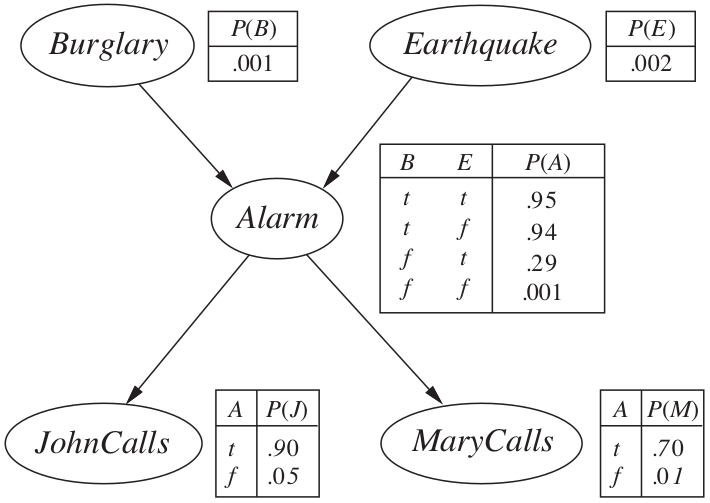
\includegraphics[scale=0.25]{bayesnet}
    \end{center}
\end{frame}
\begin{frame}{Probabilistic Graphical Models}
    \pause
    \begin{definition}
        A Markov Random Field (MRF), or a Markov network, is an undirected PGM which is used when the relations between
        random variables are symmetric, rather than hierarchical, e.g. pixels in an image.
    \end{definition}
    \pause
    \begin{columns}
        \begin{column}[t]{0.2 \textwidth}
            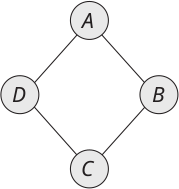
\includegraphics[scale=0.4]{mrf1}
        \end{column}
        \begin{column}[t]{0.8 \textwidth}
            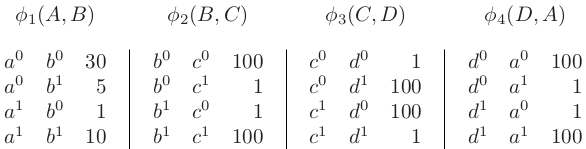
\includegraphics[scale=0.4]{mrf2}
        \end{column}
    \end{columns}
\end{frame}
\subsection{The Problem}
\begin{frame}{Belief Propagation}
    content...
\end{frame}
\begin{frame}{``Loopy'' Belief Propagation}
    content...
\end{frame}
\begin{frame}
    \begin{itemize}
        \item How far is the steady-state belief from the correct posterior when the update rules (equations 2.7-2.8) are applied in a loopy network?
        \item What are the conditions under which the BU assignment equals the MM assignment when the update rules are applied in a loopy network?
        \item What are the conditions under which the BR assignment equals the MAP assignment when the update rules are applied in a loopy network?
    \end{itemize}
\end{frame}
\section{Content}
%\begin{frame}
%    \begin{tikzpicture}
%    
%    % Define nodes
%    \node[obs]                               (y) {$y$};
%    \node[latent, above=of y, xshift=-1.2cm] (w) {$\mathbf{w}$};
%    \node[latent, above=of y, xshift=1.2cm]  (x) {$\mathbf{x}$};
%    \node[latent, right=2cm of y]            (t) {$\tau$};
%    
%    % Connect the nodes
%    \edge {x,w,t} {y} ; %
%    
%    % Plates
%    \plate {yx} {(x)(y)} {$N$} ;
%    \plate {} {(w)(y)(yx.north west)(yx.south west)} {$M$} ;
%    
%    \end{tikzpicture}
%\end{frame}
\section{Conclusion}

\end{document}
